\documentclass[times, utf8, zavrsni, numeric]{fer}
\usepackage{booktabs}
\usepackage{textcomp}
\usepackage{listings}
\lstset{
    language=C,
    tabsize=2,
    basicstyle=\footnotesize\ttfamily,
    numbers=left,
    numbersep=0em,
    xleftmargin=2em,
    frame=single,
    framexleftmargin=2em,
    breaklines=true,
    breakatwhitespace=false,
    showstringspaces=false
}

\begin{document}

% Navedite broj rada.
\thesisnumber{439}

% Navedite naslov rada.
\title{Programska potpora za prikupljanje i obradu senzorskih podataka na CubeSat nanosatelitu}

% Navedite vaše ime i prezime.
\author{Petar Sušac}

\maketitle

% Ispis stranice s napomenom o umetanju izvornika rada. Uklonite naredbu \izvornik ako želite izbaciti tu stranicu.
\izvornik

% Dodavanje zahvale ili prazne stranice. Ako ne želite dodati zahvalu, naredbu ostavite radi prazne stranice.
\zahvala{}

\tableofcontents

\chapter{Uvod}
    Projekt FERSAT, koji se od 2018. godine provodi na Fakultetu elektrotehnike i računarstva, uključuje izradu i lansiranje CubeSat satelita te korištenje satelita u svrhu prikupljanja informacija o svjetlosnom zagađenju i debljini ozonskog omotača. Satelit u izradi dimenzija je približno 10 cm x 10 cm x 10 cm, volumena jedne litre i ne teži od 4/3 kilograma, što ga svrstava u skupinu satelita formata CubeSat 1U \cite{fersat_stranica_projekta}. Očekivani životni vijek satelita je 3 godine, a bit će postavljen u Zemljinoj orbiti na visini između 500 i 600 kilometara. Slika \ref{fig:fersat} prikazuje planirani izgled satelita.
    
    \begin{figure}[htb]
        \centering
        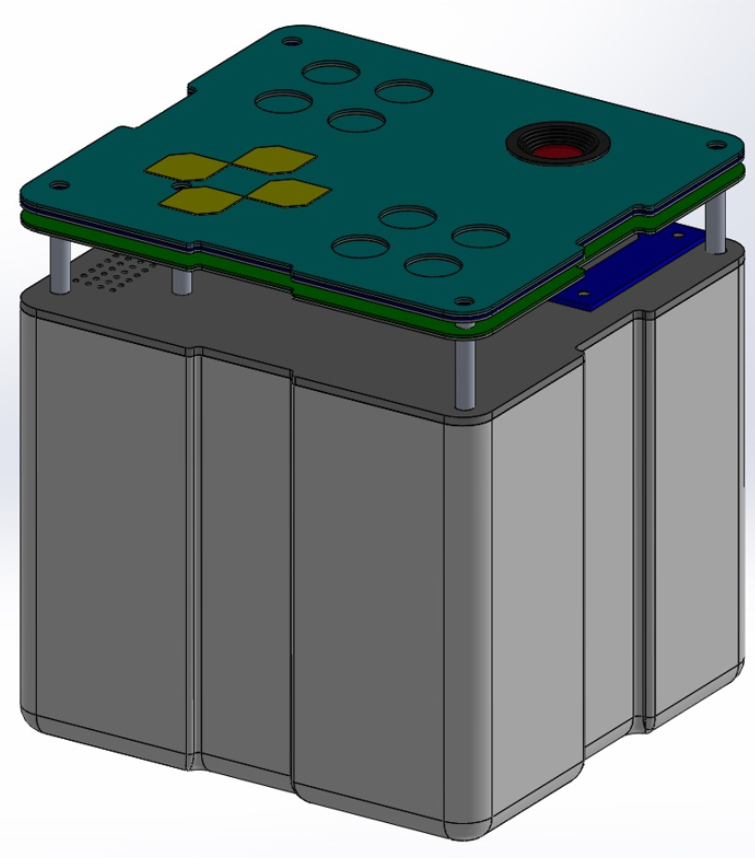
\includegraphics[height=7cm]{slike/fersat.png}
        \caption{Skica planiranog izgleda FERSAT-a. Prikazani su korisni teret \engl{payload} i platforma \engl{bus} \cite{fersat_stranica_projekta}}
        \label{fig:fersat}
    \end{figure}
    
    Planirani korisni teret \engl{payload} FERSAT-a podijeljen je na tri podsustava:

    \begin{itemize}
        \item kamera za snimanje površine Zemlje i zemaljskog horizonta,
        \item detektori svjetla u vidljivom i ultraljubičastom dijelu spektra za mjerenje svjetlosnog onečišćenja i debljine stupca ozona,
        \item komunikacijski sustav u radijskom X-pojasu (10.45 GHz) za prijenos podataka na Zemlju.
    \end{itemize}

    Radom korisnog tereta upravlja \textit{Payload Data Handler} (PDH) računalo. Zadaća je PDH računala prikupiti podatke iz senzorskog podsustava i kamere, pohraniti ih u trajnu memoriju \engl{non-volatile memory} te poslati prikupljene podatke na Zemlju korištenjem komunikacijskog podsustava. Kao PDH računalo odabran je mikrokontroler STM32L471VGT6 proizvođača ST Microelectronics.

    Za rad ostalih podsustava satelita koji nisu direktno vezani uz koristan teret (npr. upravljanje položajem satelita, slanje telemetrijskih podataka na Zemlju) brine se \textit{Command and Data Handler} (CDH) računalo. CDH računalo također upravlja napajanjem korisnog tereta i šalje naredbe PDH računalu. Komunikacija CDH i PDH računala odvija se korištenjem sučelja CAN (\textit{Controller Area Network}). Konkretno CDH računalo u trenutku pisanja ovog teksta još nije odabrano.

    Slika \ref{fig:fersat_blok} prikazuje blok dijagram cijelog sustava. U okviru ovog rada razvijena je programska potpora PDH računala za prikupljanje i obradu podataka senzorskog podsustava.
    
    \begin{figure}[htb]
        \centering
        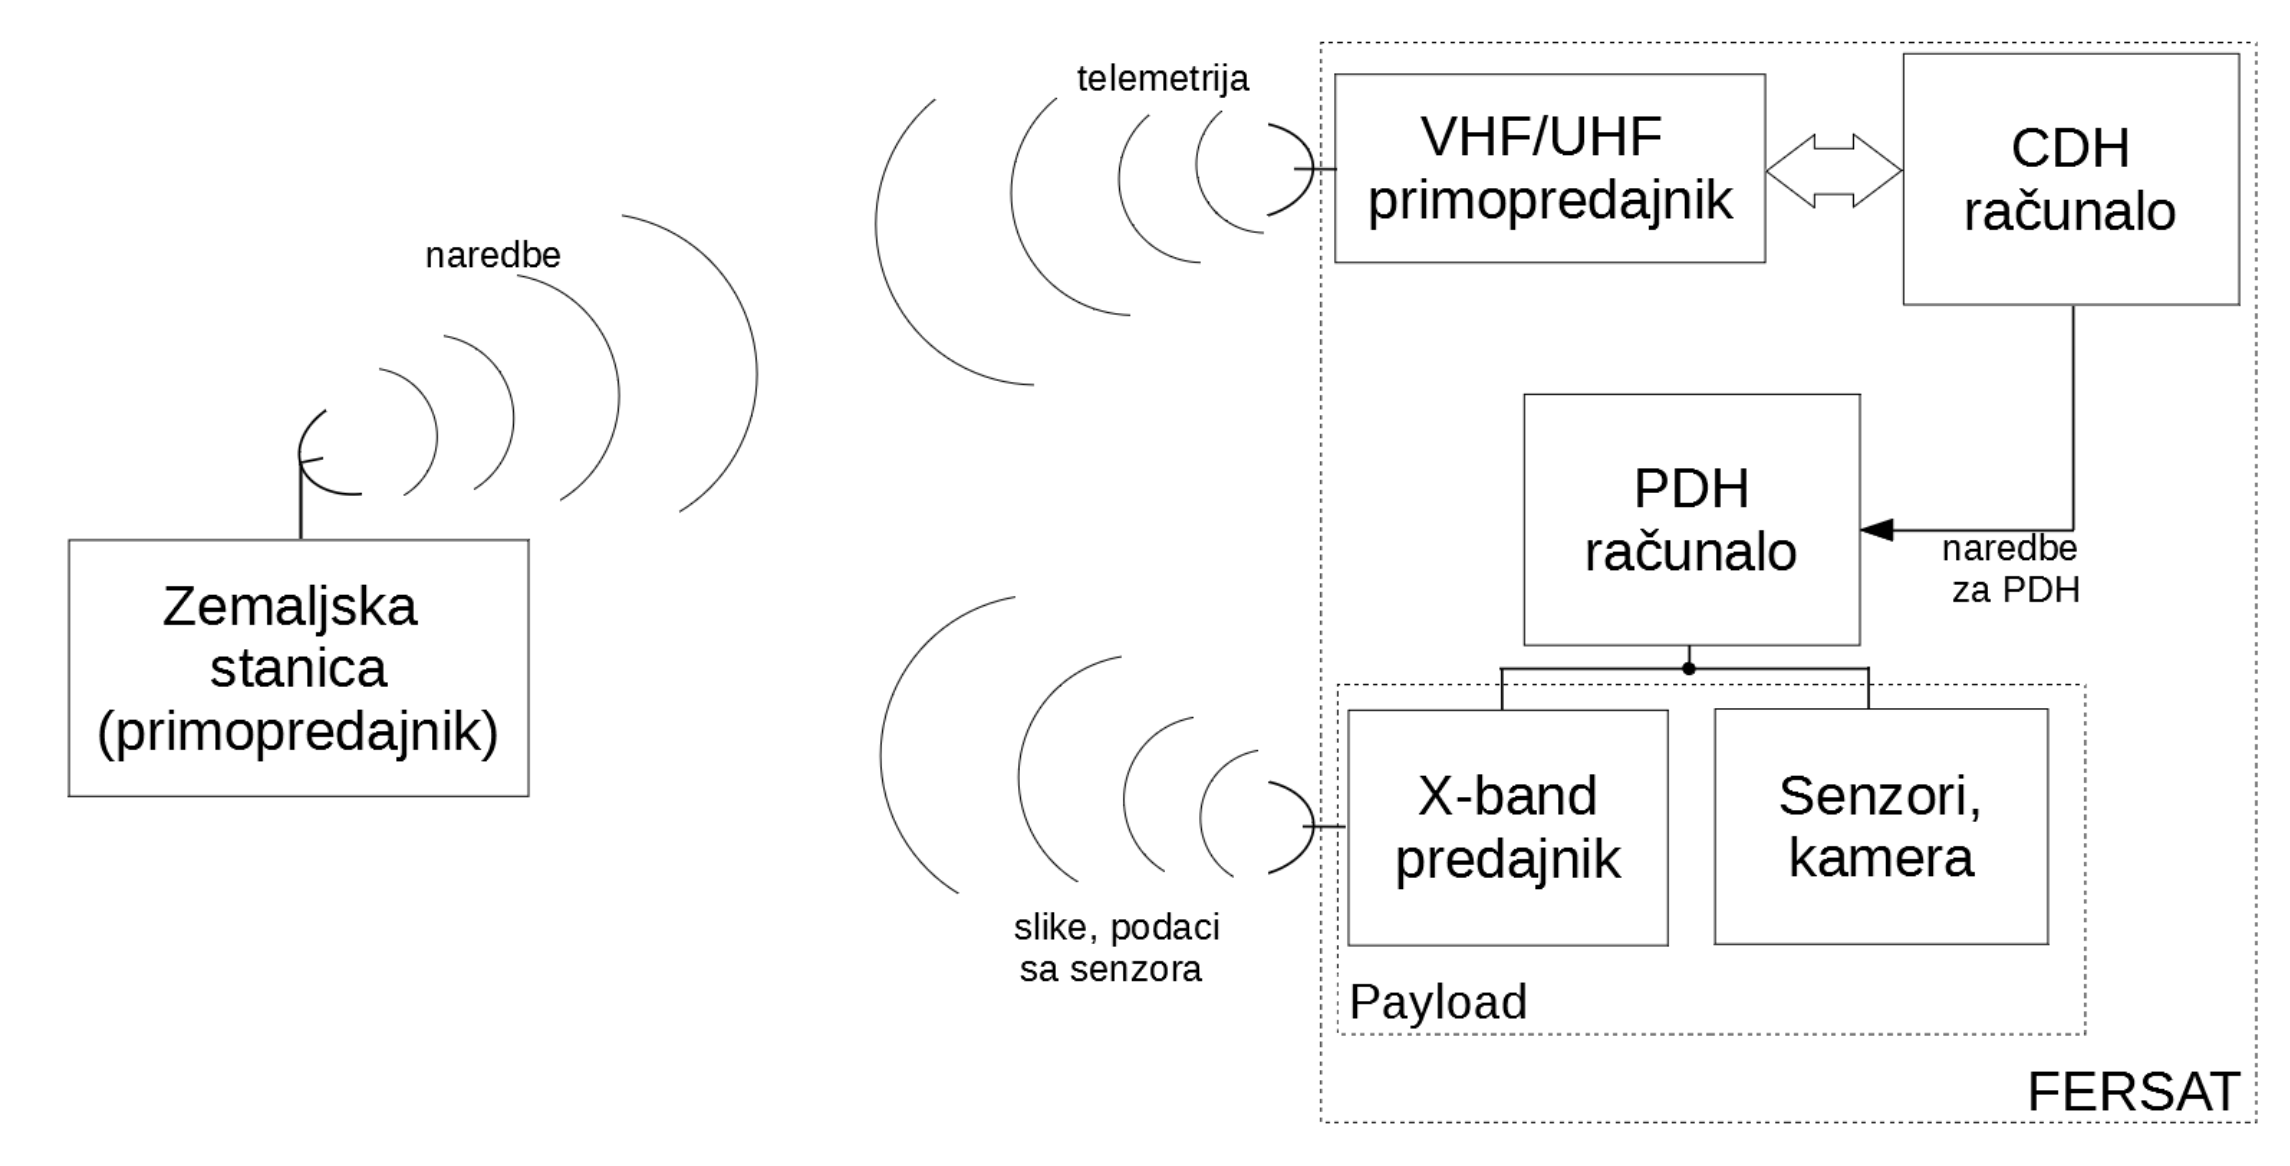
\includegraphics[width=\textwidth]{slike/fersat_blok_dijagram.png}
        \caption{Blok dijagram FERSAT-a i komunikacija sa zemaljskom postajom \cite{diplomski_goran_petrak}}
        \label{fig:fersat_blok}
    \end{figure}

    Senzorski podsustav ima dvije temeljne zadaće. Prva od njih je korištenjem fotosenzora koji rade u vidljivom dijelu elektromagnetskog spektra prikupiti podatke na temelju kojih će biti moguće odrediti udio LED rasvjete u naseljenim mjestima u odnosu na konvencionalnu natrijevu, metal-halidnu i fluorescentnu javnu rasvjetu. U sklopu projekta FERSAT već je  razvijen algoritam koji na temelju obrade signala multispektralnog svjetla sa Zemlje može odrediti ovu informaciju \cite{diplomski_jakov_tutavac}. Mjerenje udjela LED rasvjete zanimljivo je zbog mogućih negativnih utjecaja plavog svjetla na ljudsko zravlje, koje LED rasvjeta emitira u znatno većem intenzitetu nego konvencionalna \cite{falchi_light_pollution}.

    Druga je zadaća senzorskog podsustava mjerenje propusnosti i refleksije atmosfere za ultraljubičasto svjetlo u svrhu određivanja debljine ozonskog omotača. Za mjerenje se koriste PureB detektori ultraljubičastog zračenja razvijeni na FER-u \cite{diplomski_filip_bogdanovic} i algoritmi razvijeni za tu namjenu \cite{zavrsni_kristian_stepancic}. Uspješna mjerenja po prvi put bi potvrdila mogućnost korištenja ove tehnologije u mjerenjima debljine ozonskog omotača iz svemira.

    Upravljačko sklopovlje potrebno za rad PDH računala već je razvijeno \cite{zavrsni_filip_juric}. Tiskana pločica PDH računala, osim mikrokontrolera STM32L471VGT6, sadrži i vanjsku \textit{Flash} memoriju, sustav za napajanje, sklop za kontrolu izvođenja programa \engl{watchdog}, upravljački sklop za CAN komunikaciju i konektore za povezivanje s ostalim dijelovima sustava. PDH pločica bit će smještena ispod senzorske pločice, u takozvanoj \textit{stack-up} konfiguraciji (slika \ref{fig:fersat_3d}).

    \begin{figure}[htb]
        \centering
        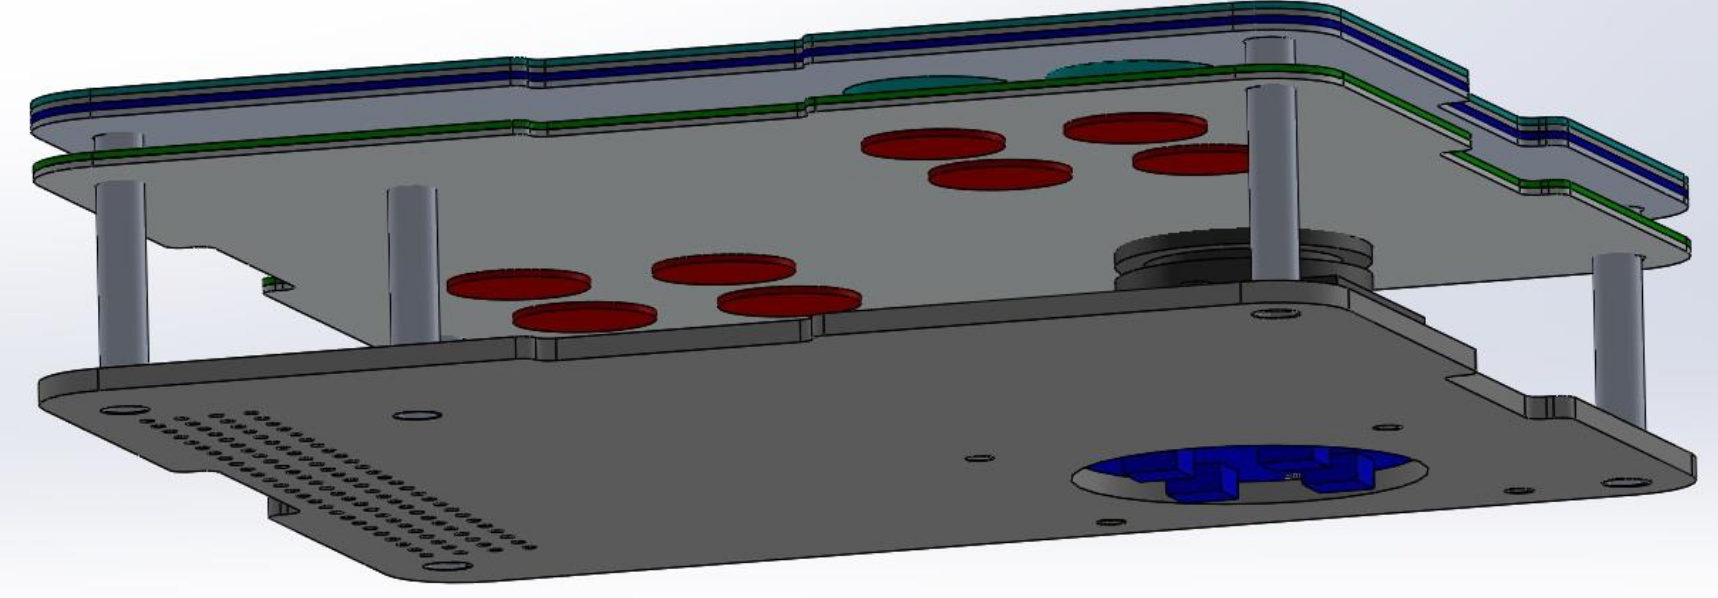
\includegraphics[width=\textwidth]{slike/fersat_3d.png}
        \caption{Trodimenzionalni model korisnog tereta FERSAT-a. PDH računalo smješteno je na donjoj pločici, a senzorski podsustav na srednjoj \cite{zavrsni_filip_juric}}
        \label{fig:fersat_3d}
    \end{figure}

    Također, u sklopu projekta FERSAT razvijen je i dio programske potpore PDH računala \cite{diplomski_goran_petrak}. No, kako je u međuvremenu došlo do promjene izbora mikrokontrolera PDH računala i promjene dijela sklopovlja senzorskog podsustava, dijelove te programske potpore bilo je potrebno prilagoditi ili ponovno razviti.
    
    Nastavak rada strukturiran je na sljedeći način. U poglavlju 2 opisano je komunikacijsko sučelje između mikrokontrolera STM32L471VGT6 i senzorskog podsustava (SPI - \textit{Serial Peripheral Interface}). Detaljan opis sklopovlja senzorskog podsustava dan je u poglavlju 3. U poglavlju 4 opisani su razvijeni upravljački programi za pojedine sklopovske komponente, cjelokupna programska potpora za senzorski podsustav, i integracija s ostalim dijelovima programske potpore PDH računala korištenjem operacijskog sustava za rad u stvarnom vremenu FreeRTOS.

\chapter{Sučelje za komunikaciju sa senzorskim podsustavom}
Komponente senzorske pločice FERSAT-a, odnosno analogno-digitalni pretvornik (ADC) ADS131M08 i temperaturni senzori ADT7301 komuniciraju s PDH računalom putem sučelja SPI. S obzirom da se pri razvoju programske potpore PDH računala koriste \textit{Low-Level} biblioteke, za ispravnu implementaciju upravljačkih programa nužno je razumijevanje strukture i načina rada SPI periferije izabranog mikrokontrolera. U nastavku ovog poglavlja dan je općeniti opis SPI protokola i opis SPI periferije porodice mikrokontrolera STM32L4.

\section{SPI protokol}
\textit{Serial Peripheral Interface} (SPI) sinkrono je serijsko komunikacijsko sučelje, razvijeno u tvrtki Motorola. S obzirom da SPI sučelje omogućava brzinu prijenosa do nekoliko desetaka Mbit/s, obično se koristi za prijenos signala visokih frekvencija između računala ili mikrokontrolera i periferijskih sklopova. Podaci se prenose između jedne upravljačke jedinice \engl{master} i više upravljanih jedinica \engl{slave} korištenjem četiri prijenosne linije: SCLK (\textit{Serial Clock}), MISO (\textit{Master Input Slave Output}), MOSI (\textit{Master Output Slave Input}) i CS (\textit{Chip Select}, ponekad se naziva i \textit{Slave Select}). Signal takta pogoni \textit{master} uređaj, a pomoću linije CS \textit{master} uređaj odabire koji \textit{slave} uređaj smije komunicirati preko linija MISO i MOSI. Slika \ref{fig:spi} prikazuje tipičan način spajanja uređaja SPI sučeljem, u konfiguraciji jednog \textit{master} uređaja i tri \textit{slave} uređaja.

\begin{figure}[htb]
	\centering
	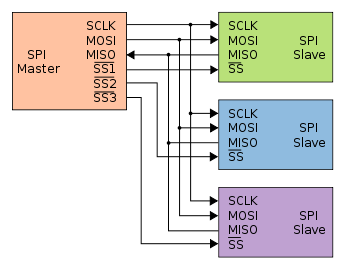
\includegraphics[height=7cm]{slike/spi.png}
	\caption{Povezivanje uređaja SPI sučeljem \cite{spi_wikipedia}}
	\label{fig:spi}
\end{figure}

Postoje 4 temeljna načina rada \engl{modes} SPI sučelja, a razlikuju se po polaritetu signala takta \engl{Clock Polarity, CPOL} i  načinu čitanja podatka sa strane master uređaja \engl{Clock Phase, CPHA}. CPOL određuje logičku razinu u koju će signal takta poprimiti u neaktivnom stanju \engl{idle state}. CPOL=0 će postaviti nisku razinu, a CPOL=1 visoku. CPHA određuje na koji brid signala takta će \textit{master} uređaj čitati podatak koji se nalazi na liniji. CPHA=0 obično znači da će to biti prvi brid, a CPHA=1 drugi. Ovisno o postavci CPOL, taj brid može biti rastući ili padajući. Ako je CPOL=0 prvi brid će biti rastući, a ako je CPOL=1, prvi brid će biti padajući. Slika \ref{fig:spi_cpol_cpha} prikazuje vremenske odnose za različite postavke CPOL i CPHA.

\begin{figure}[htb]
	\centering
	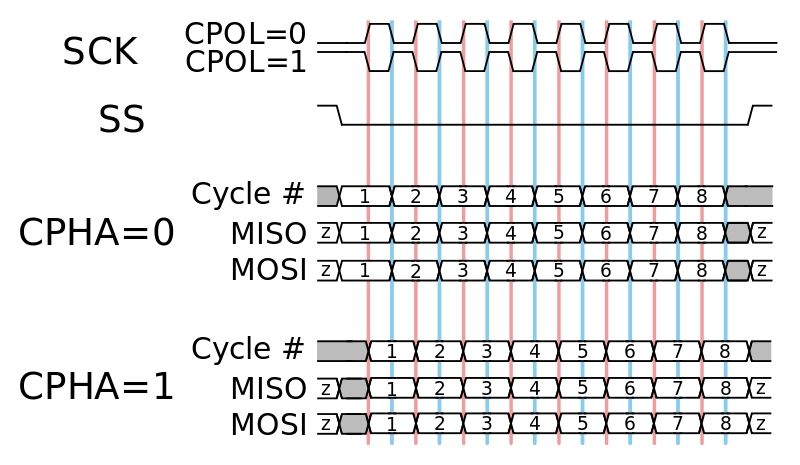
\includegraphics[height=7cm]{slike/spi_cpol_cpha.png}
	\caption{Vremenski dijagram SPI prijenosa s različitim postavkama CPOL i CPHA. Crvene linije označavaju prvi, a plave drugi brid  signala takta. \cite{spi_wikipedia}}
	\label{fig:spi_cpol_cpha}
\end{figure}

\section{Struktura SPI periferije STM32L4}
Slika \ref{fig:stm32l4_spi} prikazuje blok dijagram SPI periferije porodice mikrokontrolera STM32L4 \cite{stm32l4_manual}.

\begin{figure}[htb]
	\centering
	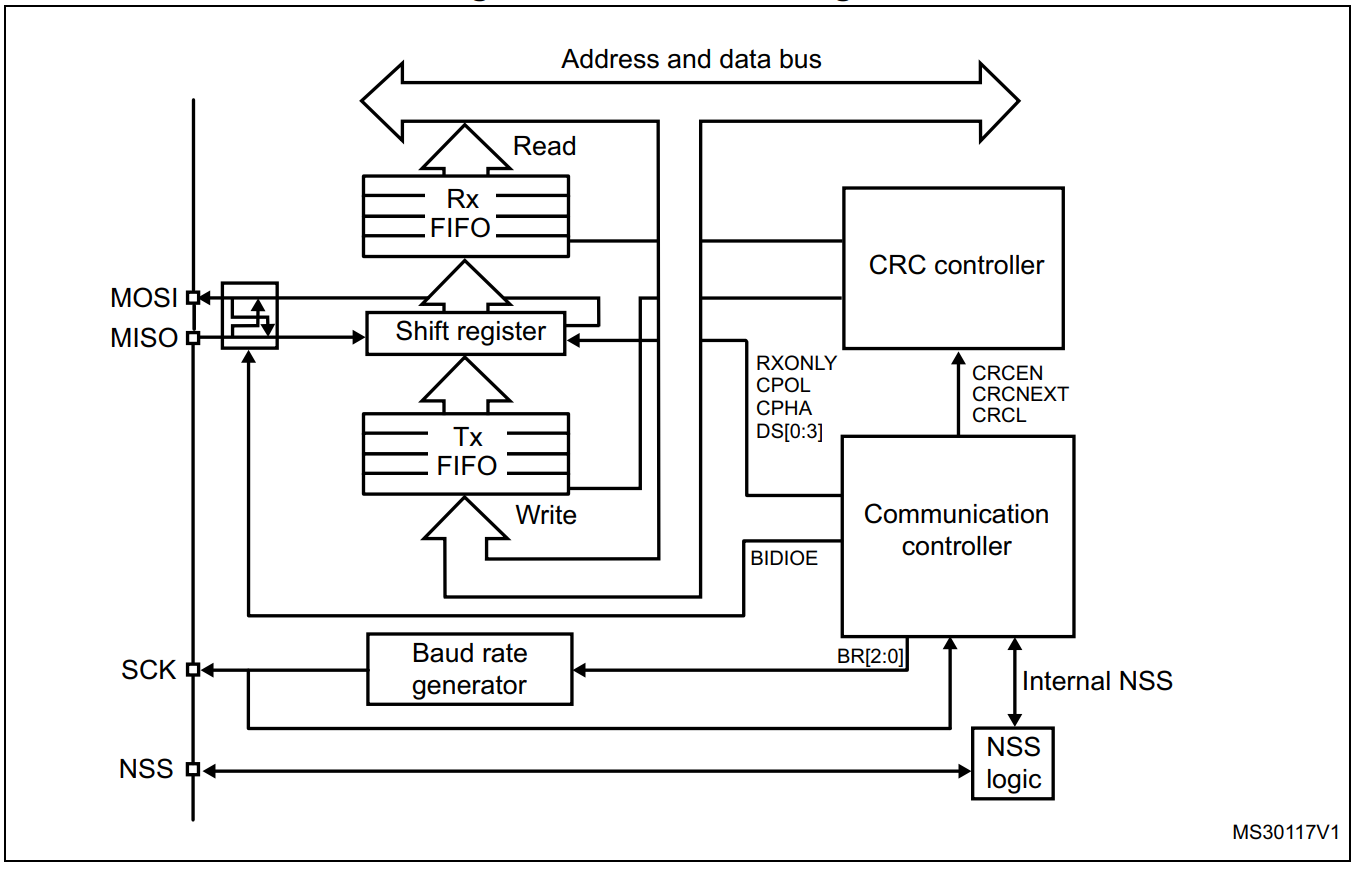
\includegraphics{slike/STM32L4_SPI_blok_dijagram.png}
	\caption{Blok dijagram SPI periferije STM32L4 \cite[str.~1451]{stm32l4_manual}}
	\label{fig:stm32l4_spi}
\end{figure}

Primanje podataka odvija se na način da riječ koja se prima po MISO liniji prvo ulazi u posmačni registar \engl{shift register}, pri čemu se na svaki period SPI takta posmiče za jedno mjesto. Kada je primljena cijela riječ, ona se na sljedeći brid takta prebacuje na kraj reda Rx FIFO \textit{First In First Out}, pri čemu se postavlja zastavica RXNE (\textit{Receiver Buffer Not Empty}) u registru stanja SPI periferije(SPIx\_SR). Prvom podatku u redu programski se može pristupiti preko SPI podatkovnog registra (SPIx\_DR). Čitanje ovog registra automatski čisti zastavicu RXNE ukoliko je popunjeno manje od četvrtine maksimalnog kapaciteta reda.

Slanje podataka odvija se na sličan način. Riječ upisana u SPIx\_DR sprema se na kraj reda Tx FIFO. Prva riječ u redu prebacuje se u posmačni registar, te se izlazni bit pri svakom posmaku šalje po liniji MOSI. Ako Tx FIFO sadrži manje podataka od pola svog kapaciteta, postavlja se zastavica TXE (\textit{Transmitter Buffer Empty}). Postavljanje te zastavice signalizira programu da se sljedeća riječ može upisati u red.

Važno je naglasiti da SPIx\_DR nije fizički registar, već se radi o virtualnom registru koji služi za pristup redovima Rx FIFO i Tx FIFO. Pisanje u ovaj registar umeće podatak na kraj reda Tx FIFO, a čitanje sadržaja registra vraća prvi podatak u redu Rx FIFO. Oba reda su veličine 32 bita, odnosno mogu primiti 4 8-bitne riječi. Nivo popunjenosti, tj. broj 8-bitnih riječi u redu može se dobiti čitanjem bitova FTLVL[1:0] za Tx FIFO, odnosno FRLVL[1:0] za Rx FIFO u SPIx\_SR. 

SPI kontroler može raditi s duljinama riječi od 4 do 16 bita. U izradi ovog rada korištena je duljina riječi 8 bita.

Kontroler omogućuje hardversko izračunavanje CRC zaštitnog koda. Ova je mogućnost nakon reseta isključena, no može se omogućiti postavljanjem bita CRCEN u registru SPIx\_CR1. Tada će pogreška u prijenosu koju otkrije CRC biti signalizirana postavljanjem zastavice CRCERR u registru SPIx\_SR.

\section{Postupak slanja i primanja podataka}
%TODO: inicijalizacija?

SPI sučelje može funkcionirati u nekoliko načina rada s obzirom na smjer komunikacije. Ti načini rada su: \textit{Full Duplex Master, Full Duplex Slave, Half Duplex Master, Half Duplex Slave, Simplex Receive Only} i \textit{Simplex Transmit Only}. U upravljačkim programima izrađenim u sklopu ovog rada korišten je način rada \textit{Full Duplex Master}, pa će zato u nastavku ovog potpoglavlja biti opisan postupak kojeg upravljački program mora izvršiti za ispravnu komunikaciju u tom načinu rada.

Važno je naglasiti da je u \textit{Full Duplex Master} načinu rada signal SPI takta određen slanjem podataka. SPI kontroler počinje generirati signal takta upisom prve riječi podatka u podatkovni registar, te nastavlja generirati signal takta dok sve riječi nisu poslane. Ako je zadnja riječ poslana i nema novih riječi u redu Tx FIFO, kontroler prestaje s generiranjem takta do sljedećeg upisa u podatkovni registar.

Upravljački program mora slijediti sljedeću proceduru\footnote{Ova procedura je prilagođena verzija procedure opisane u priručniku mikrokontrolerske porodice STM32F4 \cite[str.~887]{stm32f4_manual}.}:
\begin{enumerate}
	\item Omogućiti SPI postavljanjem bita SPE u registru SPIx\_CR1.
	\item Upisati prvu riječ za slanje u podatkovni registar.
	\item Čekati dok se ne postavi zastavica TXE i zatim upisati sljedeću riječ u podatkovni registar. Čekati dok se ne postavi zastavica RXNE i zatim pročitati riječ iz podatkovnog registra. Ponavljati ovaj korak do (uključivo) predzadnje pročitane riječi.
	\item  Čekati dok se ne postavi zastavica RXNE i pročitati zadnju riječ iz podatkovnog registra.
\end{enumerate}

Čekanje zastavice TXE prilikom upisa druge riječi nije obavezno jer će ona sigurno biti postavljena, odnosno Tx FIFO sigurno može primiti dvije 8-bitne riječi. Međutim, čekanje je potrebno za svaki sljedeći upis.

Gornja procedura implementirana je funkcijom \texttt{SPI\_TransmitReceive()}, koja pruža praktično sučelje za SPI prijenos po uzoru na HAL biblioteke.

\begin{lstlisting}
void SPI_TransmitReceive(SPI_TypeDef *SPIx, uint8_t len, uint8_t *tx_buffer, uint8_t *rx_buffer) 
{
	LL_SPI_Enable(SPIx);
	
	LL_SPI_TransmitData8(SPIx, tx_buffer[0]);
	for (int i = 0; i < len - 1; i++) {
		while ( !LL_SPI_IsActiveFlag_TXE(SPIx) );
		LL_SPI_TransmitData8(SPIx, tx_buffer[i + 1]);
		while ( !LL_SPI_IsActiveFlag_RXNE(SPIx) );
		rx_buffer[i] = LL_SPI_ReceiveData8(SPIx);
	}
	
	while ( !LL_SPI_IsActiveFlag_RXNE(SPIx) );
	rx_buffer[len - 1] = LL_SPI_ReceiveData8(SPIx);
}
\end{lstlisting}

Ako je nakon dovršenog SPI prijenosa potrebno staviti mikrokontroler u način rada male potrošnje, tada treba na ispravan način onemogućiti SPI. U nekim drugim SPI načinima rada potrebno je onemogućiti SPI nakon svakog prijenosa, npr. ako u \textit{Receive Only Master} načinu rada mikrokontroler komunicira sa sklopom koji kontinuirano šalje podatke, kako bi se spriječilo slanje dodatnih neželjenih podataka. U \textit{Full Duplex} načinu rada to obično nije potrebno, međutim dobra je praksa slijediti pravilnu proceduru za onemogućavanje SPI sučelja nakon završetka prijenosa kako bi se spriječila korupcija zadnje poslane riječi. Procedura za onemogućavanje je:

\begin{enumerate}
	\item Čekati dok se ne isprazni odlazni red (TX FIFO) provjerom bitova FTLVL[1:0] u SPI statusnom registru.
	\item Čekati dok se ne spusti zastavica BSY u SPI statusnom registru.
	\item Onemogućiti SPI čišćenjem bita SPE u registru CR1.
\end{enumerate}

Ova je procedura implementirana funkcijom \texttt{SPI\_Disable()}:

\begin{lstlisting}
void SPI_Disable(SPI_TypeDef *SPIx) {
	while (LL_SPI_GetTxFIFOLevel(SPIx) != LL_SPI_TX_FIFO_EMPTY);
	while (LL_SPI_IsActiveFlag_BSY(SPIx));
	LL_SPI_Disable(SPIx);
}
\end{lstlisting}

Tijekom uhodavanja SPI komunikacije sa sklopom ADT7301 uočena je greška u implementaciji HAL biblioteke za rad s SPI periferijom kada je SPI u \textit{Receive Only} načinu rada. Naime, u navedenom načinu rada potrebno je očistiti SPE bit točno jedan ciklus SPI takta nakon primitka predzadnje riječi kako bi se spriječilo da uređaj koji šalje podatak inicira prijenos nove riječi \cite[str.~894]{stm32f4_manual}. HAL funkcija \texttt{HAL\_SPI\_TransmitReceive()} čisti SPE bit tek nakon primitka zadnje riječi, zbog čega senzor šalje još jednu riječ, pa ukupna duljina prijenosa iznosi 24 bita umjesto 16. Također, funkcija čeka da se sklopovski očisti zastavica RXNE prije nego što završi s izvođenjem, a s obzirom da se zadnja riječ nikad ne pročita, zastavica uvijek ostaje postavljena. Zbog toga funkcija uvijek čeka do isteka \textit{timeout} intervala, što nije poželjno ponašanje. No, to nije predstavljalo problem u daljnem tijeku izrade ovog rada, jer su za razvoj korištene LL biblioteke i \textit{Full Duplex} način rada.

\section{Prijenos podataka korištenjem DMA sklopa}

Prijenos podataka SPI sučeljem između PDH računala i AD pretvornika podrazumijeva slanje relativno velike količine podataka, što može prilično dugo trajati, ovisno o brzini prijenosa. Zato je korisno koristiti DMA (\textit{Direct Memory Access}) sklop za prijenos podataka između SPI periferije i memorije. Za vrijeme DMA prijenosa procesor je rasterećen pa može obavljati druge korisne zadatke, odnosno moguće je ostvarenje neblokirajućih funkcija za SPI prijenos. Dodatna prednost je i smanjenje ukupnog trajanja komunikacije. Naime, kada se SPI komunikacija obavlja programski, program mora prvo upisati odlaznu riječ u podatkovni registar, zatim čekati primitak cijele dolazne riječi, te pročitati riječ prije upisa sljedeće riječi. To ponekad može uzrokovati diskontinuirani prijenos, odnosno periode čekanja između slanja dvije riječi. \cite[str.~890]{stm32f4_manual} Korištenjem DMA slanje i primanje može se obavljati istovremeno, što eliminira ovaj problem.

Odabrani mikrokontroler sadrži dva DMA sklopa, a svaki od njih ima 7 prijenosnih kanala. Periferija SPI3 spojena je na sklop DMA2, i to tako da je linija zahtjeva za dolazni prijenos (RX) spojena na kanal 1, a odlazni prijenos (TX) na kanal 2. 

Prije korištenja DMA sklopa potrebno je obaviti određenu inicijalizaciju. Većina te inicijalizacije, kao što je omogućavanje prekida, postavljanje smjera prijenosa i slično, može se obaviti u alatu CubeMX, pa će ovdje biti opisani samo oni koraci koji se moraju obaviti nakon CubeMX inicijalizacije, s obzirom da su oni posebno važni za razvoj programske potpore. Ne smije se zaboraviti ni inicijalizacija SPI periferije, kako bi ona mogla slati zahtjeve za DMA prijenos. U nastavku je opisana potrebna procedura i programski kod kojim se ta procedura implementira, te je uz svaki korak procedure naveden broj linije koja implementira taj korak.

\begin{enumerate}
	\item Postaviti adresu periferije za svaki kanal upisom u registar CPAR. Ova se adresa neće inkrementirati nakon svakog prijenosa. (2)
	\item Postaviti adresu memorije za svaki kanal upisom u registar CMAR. Ova će adresa biti inkrementirana nakon svakog prijenosa, a iznos inkrementa ovisi o veličini riječi. (3)
	\item Omogućiti \textit{Transfer Complete} (TC) prekide za svaki kanal upisom bita TCIE u registru CCR. (4)
	\item Postaviti duljinu prijenosa, odnosno broj riječi koje se trebaju prenijeti za svaki kanal upisom u registar CNDTR. (8)
	\item Omogućiti SPI RX zahtjeve za DMA prijenos upisom bita RXDMAEN u SPI registru CR2. (12)
	\item Omogućiti odgovarajuće DMA kanale upisom bita EN u registru CCR za svaki kanal. (16, 17)
	\item Omogućiti SPI TX zahtjeve za DMA prijenos upisom bita TXDMAEN u SPI registru CR2. (21)
	\item Omogućiti prekide koje okidaju SPI zastavice RXNE i TXE upisom bitova RXNEIE odnosno TXEIE u SPI registru CR2. (25, 26)
\end{enumerate}

\begin{lstlisting}
void DMA_Channel_Init(DMA_TypeDef *DMAx, uint32_t channel, uint32_t periph_addr, uint8_t *mem_addr) {
	LL_DMA_SetPeriphAddress(DMAx, channel, periph_addr);
	LL_DMA_SetMemoryAddress(DMAx, channel, (uint32_t)mem_addr);
	LL_DMA_EnableIT_TC(DMAx, channel);
}

void DMA_Set_Channel_Data_Length(DMA_TypeDef *DMAx, uint32_t channel, uint32_t length) {
	LL_DMA_SetDataLength(DMAx, channel, length);
}

void SPI_Enable_DMA_Rx_Request(SPI_TypeDef *SPIx) {
	LL_SPI_EnableDMAReq_RX(SPIx);
}

void DMA_Enable_CH1_CH2(DMA_TypeDef *DMAx) {
	LL_DMA_EnableChannel(DMAx, LL_DMA_CHANNEL_1);
	LL_DMA_EnableChannel(DMAx, LL_DMA_CHANNEL_2);
}

void SPI_Enable_DMA_Tx_Request(SPI_TypeDef *SPIx) {
	LL_SPI_EnableDMAReq_TX(SPIx);
}

void SPI_Enable_RXNE_TXE_Interrupts(SPI_TypeDef *SPIx) {
	LL_SPI_EnableIT_RXNE(SPIx);
	LL_SPI_EnableIT_TXE(SPIx);
}
\end{lstlisting}

Po završetku DMA prijenosa za svaki kanal, bit će generiran \textit{Transfer Complete} (TC) prekid. Bitno je primijetiti da se prekid generira za svaki kanal posebno. U prekidnoj rutini tih prekida potrebno je očistiti zastavicu CTCFIFx (za kanal x) u DMA registru IFCR i onemogućiti odgovarajući kanal kako bi se spriječio nastavak prijenosa na sljedeći SPI zahtjev kada se postavi zastavica TXE ili RXNE. Kada završe oba prekida, potrebno je onemogućiti SPI RX i TX DMA zahtjeve. Programski kod koji obavlja ovu zadaću dan je u nastavku. S obzirom da prekidne rutine TC prekida izgledaju gotovo identično za oba kanala, navedena je samo jedna od njih.

\begin{lstlisting}
void DMA_Transfer_Complete_RX_interrupt_handler() {
	LL_DMA_ClearFlag_TC1(DMA2);
	LL_DMA_DisableChannel(DMA2, LL_DMA_CHANNEL_1);
	if (tc == 1) {
		DMA_Disable(SB_SPIx);
		tc = 0;
	} else {
		tc = 1;
	}
}

void DMA_Disable(SPI_TypeDef *SPIx) {
	SPI_Disable(SPIx);
	SPI_Disable_DMA_Requests(SPIx);
	// Postavi CS prikljucak u visoku razinu
	LL_GPIO_SetOutputPin(ADC_CS_GPIOx, ADC_CS_PIN);
	// Omoguci DRDY prekide ADC-a
	NVIC_EnableIRQ(EXTI4_IRQn);
}
\end{lstlisting}

Globalna varijabla \texttt{tc} je zastavica koja signalizira je li se prekid drugog kanala već dogodio. Tek kada oba kanala završe s prijenosom može se onemogućiti SPI i omogućiti nove prekide ADC-a.

Prije pokretanja novog prijenosa potrebno je ponoviti korake 4 do 8 inicijalizacijske procedure.


\chapter{Upravljački program za temperaturni senzor ADT7301}

\section{Opis rada sklopa ADT7301}
	Sklop ADT7301 proizvođača Analog Devices je temperaturni senzor s integriranim 13-bitnim analogno-digitalnim pretvornikom i serijskim sučeljem SPI. Omogućuje mjerenje temperature u rasponu od -40\textcelsius{} do 150\textcelsius{}, s rezolucijom 0.03125\textcelsius{} i tipičnom preciznošću \textpm{} 0.5\textcelsius{} \citep{adt7301}. Blok dijagram sklopa prikazan je na slici \ref{fig:adt7301_blok_dijagram}.
	
	\begin{figure}[htb]
		\centering
		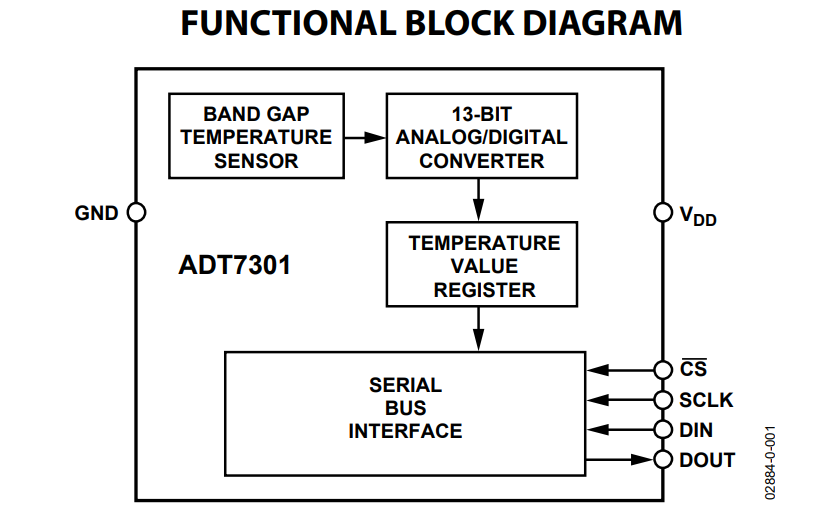
\includegraphics{slike/ADT7301_blok_dijagram.png}
		\caption{Blok dijagram sklopa ADT7301}
		\label{fig:adt7301_blok_dijagram}
	\end{figure}

	Senzor uzima mjerenja temperature svakih 1.5 sekundi, što je regulirano internim sklopom za mjerenje vremena \engl{timer}. Između dva mjerenja, napajanje analognog sklopovlja senzora je ugašeno te ono postaje neaktivno. Digitalno sklopovlje uvijek je aktivno, ali ako se pokuša pročitati vrijednost temperature više puta unutar jednog intervala mjerenja senzor će uvijek vraćati istu vrijednost (onu koju je izmjerio na početku intervala).
	
	Dodatna mogućnost sklopa je takozvani \textit{shutdown} način rada. U ovom načinu rada sklop troši vrlo malo struje (oko 1 \textmu{}A), što je korisno ako postoji dulje vremensko razdoblje u kojem se neće uzimati uzorci temperature. \textit{Shutdown} način rada omogućuje se upisom odgovarajućeg bita u kontrolni registar putem serijskog sučelja.
	
	Prilikom ispitivanja senzora u uvjetima sobne temperature, primijećeno je kako nakon nekoliko minuta kontinuiranog rada očitana temperatura počinje rasti, te može pokazivati vrijednosti čak i do 55\textcelsius{}. Zaključeno je da je navedeno posljedica zagrijavanja samog senzora. Zato je odlučeno da će se senzor između mjerenja stavljati u \textit{shutdown} način rada, kako bi se smanjila potrošnja struje, i samim time disipacija toplinske energije.

\section{SPI sučelje}
	Temperaturni senzor ADT7301 koristi SPI postavke CPOL = 1 i CPHA = 1, što znači da je takt visoke logičke razine u neaktivnom stanju i da se podatak čita na drugi brid takta (rastući).
	
	ADT7301 u stanju je istovremeno slati i primati podatke \engl{Full Duplex}. Na svojem priključku DOUT, koji je spojen na SPI liniju MOSI, sklop daje 16-bitni izlazni podatak na način da najznačajniji bit podatka izlazi prvi. Bitovi 15 i 14 su nule, bit 13 je bit predznaka, a ostali bitovi predstavljaju apsolutnu vrijednost očitane temperature. Na priključku DIN, koji je spojen na SPI liniju MISO, sklop prima 16-bitni podatak, gdje svi bitovi osim trećeg najznačajnijeg bita moraju biti nule. Treći najznačajniji bit je 1 u slučaju da se sklop želi staviti u \textit{shutdown} način rada nakon završetka ciklusa slanja, a 0 inače. Slika \ref{fig:adt7301_spi} prikazuje jedan SPI ciklus čitanja/pisanja.
	
	\begin{figure}[htb]
		\centering
		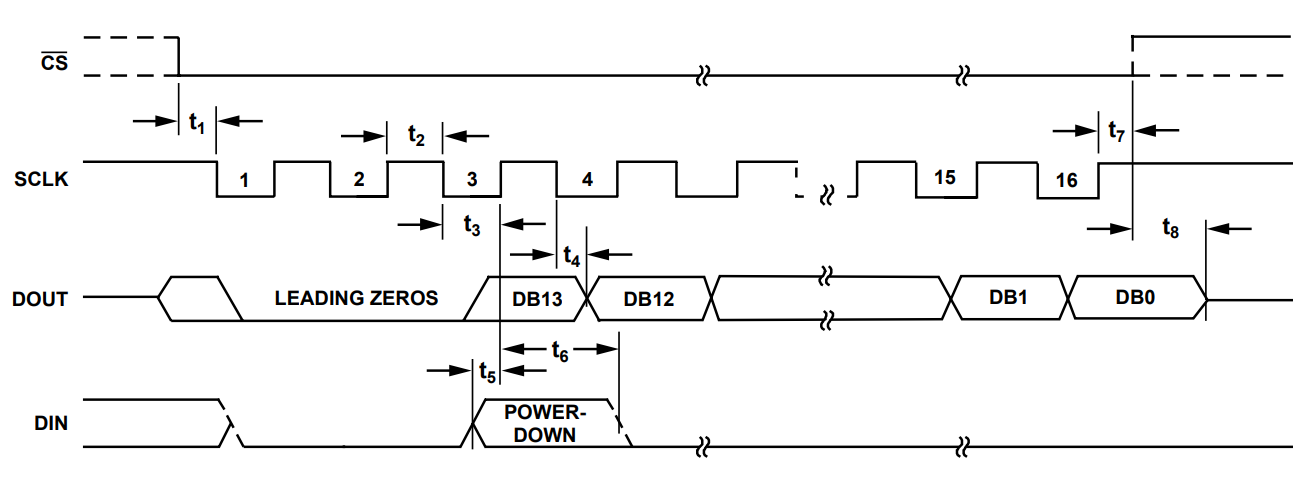
\includegraphics{slike/ADT7301_spi.png}
		\caption{Vremenski dijagram SPI komunikacije sklopa ADT7301}
		\label{fig:adt7301_spi}
	\end{figure}
	
\chapter{Zaključak}

U ovom radu opisana je razvijena programska potpora za prikupljanje i obradu senzorskih podataka nanosatelita CubeSat u okviru projekta FERSAT. Dan je kratki opis projekta FERSAT, dosadašnjih aktivnosti na projektu i objavljenih radova na koje se ovaj rad nadovezuje. Detaljno je proučeno SPI sučelje PDH računala koje se koristi za komunikaciju sa sklopovljem senzorskog podsustava i navedeni su dijelovi programske potpore koji omogućuju upravljačkim programima korištenje tog sučelja. Opisano je prethodno razvijeno sklopovlje senzorskog podsustava, navedene su najvažnije tehničke karakteristike sklopovskih komponenata za koje su razvijeni upravljački programi i opisan je način na koji te komponente koriste SPI sučelje za komunikaciju s mikrokontrolerom. Razvijeni su upravljački programi za prikupljanje podataka sa senzora, kao i programska potpora za pripremu podataka za daljnju obradu, odnosno računanje spektra signala algoritmom FFT. Programska potpora za upravljanje senzorskim podsustavom integrirana je u programsku potporu PDH računala. Razvijen je zadatak u sklopu operacijskog sustava za rad u stvarnom vremenu FreeRTOS koji upravlja aktivnostima senzorskog podsustava i zapisuje prikupljene podatke u trajnu memoriju korištenjem datotečnog sustava, te je integriran u postojeću programsku potporu. Opisan je i način mapiranja dijelova memorije u sekundarnu RAM memoriju odabranog mikrokontrolera.

Programsku potporu razvijenu u sklopu ovog rada moguće je nadograditi na nekoliko načina. Primjerice, nisu korištene naprednije mogućnosti programiranja AD pretvornika ADS131M08. Programiranjem registara AD pretvornika mogla bi se smanjiti duljina rezultata pretvorbe s 24 na 16 bita, što bi ubrzalo prijenos podataka bez gubitka preciznosti koji bi bio značajan za ovu primjenu. Bilo bi vrijedno i istražiti mogućnost povećanja frekvencije uzorkovanja. Također, nije korištena mogućnost izračunavanja CRC zaštitnog koda kako bi se podaci zaštitili od grešaka tijekom prijenosa.

Na kraju, moglo bi biti od koristi istražiti mogućnost korištenja vanjske serijske RAM memorije kako bi se riješio problem velike zauzetosti radne memorije mikrokontrolera.

\bibliography{literatura}
\bibliographystyle{fer}

\begin{sazetak}
Sažetak na hrvatskom jeziku.

\kljucnerijeci{Ključne riječi, odvojene zarezima.}
\end{sazetak}

% Navedite naslov na engleskom jeziku.
\engtitle{Software for CubeSat Nanosatellite Sensor Data Acquisition and Processing}
\begin{abstract}
Abstract.

\keywords{Keywords.}
\end{abstract}

\end{document}
